\documentclass[10pt,xcolor=svgnames,handout]{beamer} %Beamer
\usepackage{palatino} %font type
\usefonttheme{metropolis} %Type of slides
\usefonttheme[onlymath]{serif} %font type Mathematical expressions
\usetheme[progressbar=frametitle,titleformat frame=smallcaps,numbering=counter]{metropolis} %This adds a bar at the beginning of each section.
\useoutertheme[subsection=false]{miniframes} %Circles in the top of each frame, showing the slide of each section you are at

\usepackage{appendixnumberbeamer} %enumerate each slide without counting the appendix
\setbeamercolor{progress bar}{fg=Maroon!70!Coral} %These are the colours of the progress bar. Notice that the names used are the svgnames
\setbeamercolor{title separator}{fg=DarkSalmon} %This is the line colour in the title slide
\setbeamercolor{structure}{fg=black} %Colour of the text of structure, numbers, items, blah. Not the big text.
\setbeamercolor{normal text}{fg=black!87} %Colour of normal text
\setbeamercolor{alerted text}{fg=DarkRed!60!Gainsboro} %Color of the alert box
\setbeamercolor{example text}{fg=Maroon!70!Coral} %Colour of the Example block text


\setbeamercolor{palette primary}{bg=NavyBlue!50!DarkOliveGreen, fg=white} %These are the colours of the background. Being this the main combination and so one. 
\setbeamercolor{palette secondary}{bg=NavyBlue!50!DarkOliveGreen, fg=white}
\setbeamercolor{palette tertiary}{bg=NavyBlue!40!Black, fg= white}
\setbeamercolor{section in toc}{fg=NavyBlue!40!Black} %Color of the text in the table of contents (toc)

%These next packages are the useful for Physics in general, you can add the extras here. 
\usepackage{amsmath,amssymb}
\usepackage{slashed}
\usepackage{cite}
\usepackage{relsize}
\usepackage{caption}
\usepackage{subcaption}
\usepackage{multicol}
\usepackage{booktabs}
\usepackage[scale=2]{ccicons}
\usepackage{pgfplots}
\usepgfplotslibrary{dateplot}
\usepackage{geometry}
\usepackage{xspace}
\newcommand{\themename}{\textbf{\textsc{bluetemp}\xspace}}%metropolis}}\xspace}
\DeclareMathOperator{\sinc}{sinc}
\graphicspath{{./images/}}
\title{Introduction to statistics and data science}
\author[Name]{Stéphane Puechmorel \inst{$\dagger$}}
\subtitle{A hands-on approach}
\institute[uni]{\inst{$\dagger$} ENAC Dept. SINA \\ email: stephane.puechmorel@enac.fr \\ phone: 0562259503}
\date{\today} %Here you can change the date
\titlegraphic{\vspace{-0.5cm}\hfill
\includegraphics[scale=0.3]{images/ENAC-Orange.png}} %You can modify the location of the logo by changing the command \vspace{}. 

\definecolor{almond}{rgb}{0.94, 0.87, 0.8}
\definecolor{bubbles}{rgb}{0.91, 1.0, 1.0}
\newcommand{\R}{\ensuremath{\mathbb{R}}}
\newcommand{\C}{\ensuremath{\mathbb{C}}}
\newcommand{\N}{\ensuremath{\mathbb{N}}}

\begin{document}
{
\setbeamercolor{background canvas}{bg=NavyBlue!50!DarkOliveGreen, fg=white}
\setbeamercolor{normal text}{fg=white}
\maketitle
}%This is the colour of the first slide. bg= background and fg=foreground

\metroset{titleformat frame=smallcaps} %This changes the titles for small caps

\begin{frame}{Outline}
  \setbeamertemplate{section in toc}[sections numbered] %This is numbering the sections
  \tableofcontents[hideallsubsections] %You can comment this line if you want to show the subsections in the table of contents
\end{frame}




\section{Introduction}

% \begin{frame}{Objectives}
% %\underline{\textsc{Some text:}}
% % \begin{small}
% % This is some small Text. 
% % \end{small}

% % \metroset{block=fill}
% % \begin{exampleblock}{\textsc{Example block}}
% % \begin{itemize}
% %     \item You know how to do itemize
% %     \item Also here
% % \end{itemize}
% % \end{exampleblock}
% \end{frame}

%1
\begin{frame}[fragile]{Introduction to statistics and data science}
\begin{block}{Why this course ?}
\begin{itemize}
    \item<+-> Data are omnipresent in engineering and business intelligence.
    \item<+-> Understanding them can often be challenging.
    \item<+-> Statistics provides the data analyst with a rigorous framework.
\end{itemize}
\end{block}
\begin{block}{Course contents:}
\begin{itemize}
    \item<+-> Concepts from probability theory.
    \item<+-> Visual data exploration.
    \item<+-> Inferential statistics.
    \item<+-> Hypothesis testing.
\end{itemize}
\end{block}
\end{frame}

%2
\begin{frame}[fragile]{Work organization}
\begin{itemize}
    \item<+-> All lectures will include course material and exercises.
    \item<+-> The notions are illustrated using real data and statistical software.
    \item<+->Should you encounter any difficulties, please do not hesitate to inquire.
    \item<+->Personal work is essential and must be completed regularly.
\end{itemize}
\end{frame}

%3
\begin{frame}[fragile]{Software}
\begin{itemize}
    \item<+-> Two software products will be utilized during the course:
    \begin{itemize}
        \item<+-> R, that is widely recognized as the prevailing standard within the statistical community.
        \item<+-> PowerBI, a tool that is being used with increasing frequency for the collection, processing, and visualization of data. It integrates almost seamlessly with R. 
    \end{itemize}
    \item<+-> Advanced concepts will not be covered. 
    \item<+-> Feel free to install both on your personal computer. Power BI Desktop cannot share dashboards
     unless you have a paid subscription, but this is not a significant issue when learning how to use the tool. 
    \end{itemize}
\end{frame}
\documentclass[main.tex]{subfiles}
\begin{document}
\section{Visual exploration of data}
\begin{frame}
    \frametitle{An introduction to PowerBI}
\begin{block}{A report generator}
    \begin{itemize}
        \item<+-> Power BI is a reporting and data analytics tool
        that simplifies data collection, transformation, 
        and visualization tasks.
        \item<+-> It is designed to be extensible and has become
        the de facto standard in the industry.
    \end{itemize}
\end{block}
\begin{block}{What PowerBI is not}
    \begin{itemize}
        \item<+-> While it performs well in terms of data visualization,
         it is not a full-fledged statistical software.
        \item<+-> The use of a superior data transformation
         and analysis tool is a highly effective strategy.
    \end{itemize}
\end{block}    i
\end{frame}
\begin{frame}
    \frametitle{R}
\begin{block}{The workhorse of statistics}
    \begin{itemize}
        \item<+-> A free and open source piece of software.
        \item<+->R boasts implementation of nearly all developments in statistics.
        \item<+-> The number of free programs written in R is keeping increasing.
    \end{itemize}
\end{block}
\begin{block}{A companion to PowerBI}
    \begin{itemize}
        \item<+-> PowerBI can collect data from a R script.
        \item<+-> PowerBI can transform data using a R script.
        \item<+-> PowerBI can display the output of a R script. 
    \end{itemize}
\end{block}    
\end{frame}
\begin{frame}
    \frametitle{R in a nutshell}
\begin{block}{R as a desk calculator}
    \begin{itemize}
        \item<+-> Open R by double-clicking on the R icon.
        \item<+-> Simply type "2+3" and observe the result.
        \begin{figure}[htbp]
            \centering
            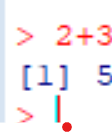
\includegraphics[scale=0.5]{R-sum.png}
            \caption{A simple sum}
            \label{<label>}
        \end{figure}
        \item<+-> A value  can be stored in
        a variable with the operator \texttt{<-}.
        \begin{figure}[htbp]
            \centering
            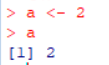
\includegraphics[scale=0.5]{variable.PNG}
            \caption{Using a variable.}
            \label{fig:variable}
        \end{figure}
    \end{itemize}
\end{block}
\end{frame}
\begin{frame}
    \frametitle{Vectors}
\begin{block}{Vectors}
    \begin{itemize}
        \item<+-> Vectors are created using the "c" (concatenate) or range operator "min:max".
        \item<+-> Try "c(0.1, 2, 3)" and "1:100".
        \item<+-> If you want a non-unit step, use the "seq(min, max, step)" command.
        \begin{figure}[htbp]
            \centering
            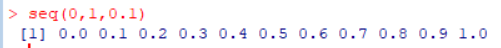
\includegraphics[scale=0.5]{seq_example.png}
            \caption{User-defined step}
            \label{fig:arbitrary_range}
        \end{figure}
        \item<+-> All the elements of a vector must be of the same type:
        numeric (double, integer, complex), logical, string.
    \end{itemize}
\end{block}
\end{frame}
\begin{frame}
    \frametitle{Vectors}
    \begin{block}{Numeric and boolean types}
        \begin{itemize}
            \item<+-> By default, a numeric value is encoded 
            as a double precision number on 64 bits. 
            \item<+-> A complex number is declared with syntax $x + yi$:
           \begin{figure}[htbp]
            \centering
            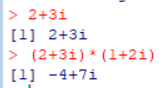
\includegraphics[scale=0.5]{complex_number.PNG}
            \caption{Complex numbers}
            \label{fig:complex_numbers}
           \end{figure}
           \item<+-> Booleans are TRUE or FALSE.
           \begin{figure}[htbp]
            \centering
            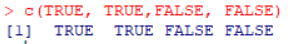
\includegraphics[scale=0.5]{boolean.PNG}
            \caption{Booleans}
            \label{fig:booleans}
           \end{figure}
        \end{itemize}
    \end{block}
\end{frame}
\begin{frame}
    \frametitle{Vectors}
    \begin{block}{Character strings}
        \begin{itemize}
           \item<+-> A string is enclosed with double or simple quotes.
           \begin{figure}[htbp]
            \centering
           
\includegraphics[scale=0.5]{string.PNG} 
            \caption{Character strings}
            \label{fig:char_strings}
           \end{figure}
           \item<+-> Any R object can be converted to an informative string with the function
           \texttt{str().}
        \begin{figure}[htbp]
            \centering
           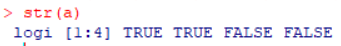
\includegraphics[scale=0.5]{str_func.PNG} 
            \caption{Str function.}
            \label{fig:str_func}
           \end{figure}
        \end{itemize}
    \end{block}
\end{frame}

\begin{frame}
    \frametitle{Vectors}
\begin{block}{Operators}
   \begin{itemize}
    \item<+->Operators and functions are applied elementwise.
     \begin{figure}[htbp]
            \centering
           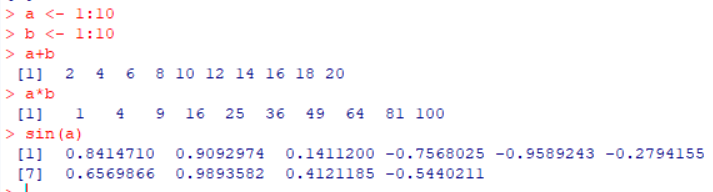
\includegraphics[scale=0.5]{vector_functions.PNG} 
            \caption{Operating on vectors.}
            \label{fig:vect_op}
           \end{figure}
    \item<+-> This is true also for comparison operators.
     \begin{figure}[htbp]
            \centering
           
\includegraphics[scale=0.5]{comparison.PNG}
            \caption{Comparison operators.}
            \label{fig:vect_comp}
           \end{figure}
   \end{itemize} 
\end{block}
\end{frame}
\begin{frame}
    \frametitle{Vectors}
    \begin{block}{Accessing elements}
        \begin{itemize}
            \item<+-> An element in a vector can be referred to by its 
            index.
     \begin{figure}[htbp]
            \centering
           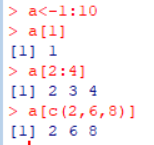
\includegraphics[scale=0.5]{elements.PNG}
            \caption{Accessing elements.}
            \label{fig:vect_elts}
           \end{figure}
           \item<+-> A selection by booleans is also possible.
           \begin{figure}[htbp]
            \centering
           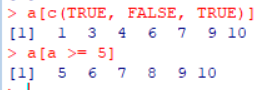
\includegraphics[scale=0.5]{bool_select.PNG}
            \caption{Boolean selection.}
            \label{fig:vect_bool}
           \end{figure}
        \end{itemize}
    \end{block}
\end{frame}
\begin{frame}
    \frametitle{Data frames}
\begin{block}{A convenient object.}
    \begin{itemize}
        \item<+-> Data frames are arrays holding observed values.
        \item<+-> Observed characteristics are in columns, observations in rows.
        \item<+-> The columns are named and can be referred to by their names.
        \begin{figure}[htbp]
            \centering
           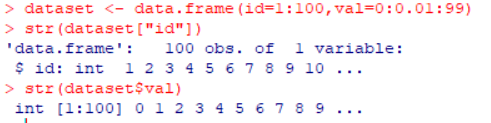
\includegraphics[scale=0.5]{dataframe.PNG}
            \caption{A data frame.}
            \label{fig:data_frame}
           \end{figure}
        \item<+-> Data frames are used by PowerBI to communicate with R.
    \end{itemize}
\end{block}
\end{frame}
\begin{frame}
    \frametitle{Passengers dataset}
    \begin{block}{Data collection}
        \begin{itemize}
            \item<+-> The dataset, collected from the site \url{https://data.europa.eu/data/datasets?locale=en}
            is stored in the file \texttt{avia\_paoc\_monthly.csv} that can be retrieved on ecampus in the folder \texttt{Datasets}.
            \item<+-> Launch PowerBI and select \texttt{Get data from other sources}.
            \item<+-> Select \texttt{Text/CSV} and open the file.
            \item<+-> A table view of the dataset appears.
        \end{itemize}
    \end{block}
\end{frame}
\begin{frame}
    \frametitle{Passengers dataset}
    \begin{block}{Data transformation}
        \begin{itemize}
            \item<+-> PowerBI offers the opportunity to transform the data.
            \begin{figure}[htbp]
                \centering
                
\includegraphics[scale=0.3]{power_bi_transform_data.png}
                \caption{Data transform.}
                \label{fig:data_transform}
            \end{figure}
            \item<+-> We are only interested in the total number of passengers carried by country, so all the rows
            below row 32 must be removed.
            \item<+-> Select \texttt{Keep rows}, then \texttt{Keep top rows} and finally enter 32. 
        \end{itemize}
    \end{block}
\end{frame}
\begin{frame}
    \frametitle{Passengers dataset}
    \begin{block}{Final transformations}
        \begin{itemize}
            \item<+-> In the first column, a description of the data includes at the end a geographic information. 
            \item<+-> Select the first column, right click on it, the select \texttt{replace values}.
            \item<+-> Copy all the text in the first cell, except the final two-characters country code.
            \item<+-> Keep the replacement text empty and click \texttt{replace}. 
        \end{itemize}
    \end{block}
   
    
\end{frame}
\begin{frame}
    \frametitle{Passengers dataset}
    \begin{block}{Transposing datasets}
        \begin{itemize}
            \item<+-> Datasets must have their values in columns.
            \item<+-> Select the tab \texttt{Transform}, then \texttt{Transpose}.
            \item<+-> Return to the \texttt{Home} tab and select \texttt{Use first row as headers}.
            \item<+-> The label of the first column is not very informative. Right click 
            on it and select \texttt{Rename}.
        \end{itemize}
    \end{block}

\end{frame}
\begin{frame}
    \frametitle{Passengers dataset}
\begin{block}{Cleaning data}
    \begin{itemize}
        \item<+-> A dataset may have blank rows. Check yours and remove
        them if needed (\texttt{Remove rows} tab).
        \item<+-> Some values may be missing. In this dataset, they are coded 
        as ":". 
        \item<+-> The column "MK" has such values. Right click on it, then use 
        \texttt{Replace values} to change ":" by "0".
        \item<+-> finally, change the type of the column to \texttt{Whole number}.
    \end{itemize}
\end{block}    
   \begin{block}{Applying transforms}
    \begin{itemize}
        \item<+-> Select the \texttt{Close and apply} to apply the transforms.
        \item<+-> It is time to save your work (tab \texttt{File}) ! 
    \end{itemize}
   \end{block} 
\end{frame}
\begin{frame}
    \frametitle{Passengers dataset}
\begin{block}{Visual exploration of the dataset}
    \begin{itemize}
        \item<+-> Return to the \texttt{Home} tab, and start populating the report.
        \item<+-> Text boxes or visual can be added. 
        \item<+-> Select a text box and enter the text you wish to start your report.
        \item<+-> Select \texttt{New visual}. A new box appears (by default a bar chart).
        \item<+-> Select \texttt{Date} in the \texttt{Data} right pane and drag 
        the \texttt{Month} field to the visual. This defines the "x" axis.
        \item<+-> You can add data to your visual by selecting columns in the \texttt{Data} pane 
        or by dragging them. 
        \item<+-> Try changing the visual and see what happens.
    \end{itemize}
\end{block}
\end{frame}
\begin{frame}
    \frametitle{Passengers dataset}
\begin{block}{Data aggregation}
    \begin{itemize}
        \item<+-> In the "passengers" dataset, there is a one-to-one mapping
        between a month and the number of passengers. 
        \item<+-> What happens if we decide to plot against the quarter ?
        \item<+-> Uncheck \texttt{Month} in \texttt{Date} on the right pane and
        select \texttt{Quarter}.
        \item<+-> The visual now displays the total number of passengers for each quarter.
        \item<+-> In the \texttt{Y axis} part of the \texttt{visualization} pane,
        try to change \texttt{Sum} to \texttt{Average}.
        \item<+-> The aggregation of values is an important feature in PowerBI.
    \end{itemize}
\end{block}
\end{frame}
\begin{frame}
    \frametitle{Passengers dataset}
\begin{block}{Measures}
    \begin{itemize}
        \item<+-> A measure is a value that can be computed from the dataset.
        \item<+-> It may be viewed as a practical implementation of a random variable,
        a concept introduced later in the course.
        \item<+-> Since measures are computed on-the-fly, they always reflect the most up-to-date dataset.
        \item<+-> Using them is a must in PowerBI.
        \item<+-> Create a \texttt{New quick measure} on the "passengers" dataset that sums the amount of 
        carried passengers by quarter for a given country (select the one you prefer).
        \item<+-> Use a visual to plot the result.
        \item<+-> Custom measures can be used, provided you know the "DAX" language.
    \end{itemize}
\end{block}
\end{frame}
\begin{frame}[fragile]
    \frametitle{PowerBI and R}
\begin{block}{R as a data source}
    \begin{itemize}
        \item<+-> Open the \texttt{Get data} tab, then select \texttt{R}.
        \item<+-> In the script box, type:
        \begin{lstlisting}{language=R}
dataset <- data.frame(x=1:100,y=runif(n=100,min=0,max=10))
        \end{lstlisting}
        \item<+-> Observe the result in PowerBI. What happens if the name \texttt{dataset} for the ouput variable is changed ?
        \item<+-> Create two data frames in the R script: what happens in PowerBI?
    \end{itemize}
\end{block}
\end{frame}
\begin{frame}[fragile]
    \frametitle{PowerBI and R}
\begin{block}{R as a data processor}
    \begin{itemize}
        \item<+-> Open the \texttt{Get data} tab, then select \texttt{Run R script}.
        \item<+-> In the script box, type:
        \begin{lstlisting}{language=R}
output <- dataset
output$z <- as.numeric(dataset$y)+1
        \end{lstlisting}
        \item<+-> A new column named \texttt{z} was added and its values are those of column \texttt{y} plus 1.
    \end{itemize}
\end{block}
\end{frame}
\begin{frame}[fragile]
    \frametitle{PowerBI and R}
\begin{block}{Visuals}
    \begin{itemize}
        \item<+-> On the \texttt{visualizations} pane, select the \texttt{R} icon.
        \item<+-> Drag the \texttt{y} field in the visual.
        \item<+-> In the script box, type:
        \begin{lstlisting}{language=R}
hist(dataset$y)
        \end{lstlisting}
        \item<+-> An histogram is displayed in the visual. 
        \item<+-> This may be useful when a given visual, like the histogram, is not implemented in PowerBI or requires a plugin.
    \end{itemize}
\end{block}
\end{frame}
\end{document}    


\documentclass[main.tex]{subfiles}
\begin{document}
\section{Probability theory}

%1
\begin{frame}
    \frametitle{A bit of history}
\begin{block}{Games of chance}
    \begin{itemize}
        \item<+-> According to popular belief, knights returning from the Crusades introduced a dice game named "Hazard."
         Although the rules were complicated, the game attracted many players.
        \item<+-> The mathematician Gerolamo Cardano, in the middle of the 16th century, starts to investigate the odds of winning
        in a game of chance. He gives the first definition of the probability of an event as the ratio of
        the number of favorable outcomes to the total number of outcomes.
        \item<+-> One century later, Pierre de Fermat and Blaise Pascal lay the first theory of probability when
        answering a question from Antoine Gombaud, a famous Parisian gambler.
    \end{itemize}
\end{block}
\end{frame}
%2
\begin{frame}
    \frametitle{A bit of history}
\begin{block}{A modern view}
    \begin{itemize}
        \item<+-> In 1933, the Russian mathematician Andrey Kolmogorov gives the first axiomatic description of probability theory.
        \item<+-> This is the approach we will take in the sequel.
    \end{itemize}
\end{block}    
\begin{block}{Challenges}
    \begin{itemize}
       \item<+-> To fully understand Kolmogorov's contribution, we must consider cases in which counting the number of favorable outcomes is insufficient.
       \item<+-> For example, take a situation where the measure of interest is a real number, such as a current or a pressure.
       \item<+-> The value itself is not discrete; only the number of times it falls within a given interval can be observed.
       \item<+-> The Fermat-Pascal approach must be extended to these cases.
    \end{itemize}
\end{block}    
\end{frame}
%3
\begin{frame}
    \frametitle{From intuition to axioms }
\begin{block}{Sample space}
    \begin{itemize}
        \item<+-> Let's consider a very simple experiment: a coin is tossed, and the outcome observed.
        \item<+-> What are the possible results ?
        \item<+-> Of course, "head" and "tails" !
        \item<+-> The \textbf{sample space} of an experiment is the set of all possible results.
        \item<+-> In the coin tossing example, it is just the set $\Omega = \{ \text{heads}, \text{tails}\}.$
        \item<+-> If a die is rolled, the sample space is $\Omega = \{ 1,2,3,4,5, 6\}.$
        \item<+-> In a physical system, $\Omega$ may be a subset of the real numbers,
        or something even more complicated.
    \end{itemize}
\end{block}    
\end{frame}
%4 
\begin{frame}
    \frametitle{From intuition to axioms}
\begin{block}{Events}
    \begin{itemize}
        \item<+-> If two coins are tossed, the sample space is 
        $\Omega = \{ HH, HT, TH, TT \}.$
        \item<+-> An \textbf{event} is a statement about the outcome of the experiment, 
        like "at least one tails was observed".
        \item<+-> The previous event is the subset $\{HT,TH,TT\}$ of $\Omega.$
        \item<+-> In probability theory, an \textbf{event} is a subset of the \textbf{sample space}.
        \item<+-> The empty set $\emptyset$ and the sample space $\Omega$ are 
        always considered as events.
    \end{itemize}
\end{block}
\end{frame}
%5 
\begin{frame}
    \frametitle{From intuition to axioms}
\begin{block}{A bit of logic}
    \begin{itemize}
        \item<+-> Assertions about events are also events:
        \begin{itemize}
            \item<+-> If $A,B$ are events, so is $A \cup B.$
            \item<+-> If $A$ is an event, the complementary set $\bar{A}$ is an event.
        \end{itemize}
        \item<+-> For the two coins tossing experiment, if $A=\{HH\},B=\{HT\}$, then
         the event $A \cup B = \{HH, HT\}$ is "the first toss is a head", while the event
        $\bar{A}=\{HT,TH,TT\}$ is "at least one tails was observed".
    \end{itemize}
\end{block}
\begin{block}{Exercise}
    \begin{itemize}
        \item<+-> Find the sample space $\Omega$ associated with the roll of a die.
        \item<+-> What are the respective subsets $A,B$ of $\Omega$ corresponding to the observations
        "the result is greater than or equal to 3","the result is an even number"?
        \item<+-> Describe the events $A\cup B$, $\bar{A}.$
    \end{itemize}
\end{block}
\end{frame}
%6
\begin{frame}
    \frametitle{Probabilities}
    \begin{block}{$\sigma$-algebras}
        \begin{itemize}
            \item<+-> Given a sample space $\Omega$, a $\sigma$-algebra of
            events is a set $\mathcal{T}$ of subsets from $\Omega$ such that:
            \begin{itemize}
                \item<+-> $\Omega \in \mathcal{T}.$
                \item<+-> If $A \in \mathcal{T}$, then $\bar{A} \in \mathcal{T}.$
                \item<+-> For any \textbf{countable} sequence $A_n$ in $\mathcal{T}$, the union
                $\bigcup_n A_n$ is in $\mathcal{T}.$
            \end{itemize}
        \end{itemize}
    \end{block}
\begin{block}{Probability measure}
    \begin{itemize}
        \item<+-> Given a $\sigma$-algebra $\mathcal{T}$ on $\Omega$, a 
        probability $P$ is a mapping that assigns to $A \in \mathcal{T}$ a real
        number $P(A) \in [0,1]$ such that:
        \begin{itemize}
        \item<+-> $P\left( \Omega \right) = 1.$
        \item<+-> For any countable sequence $A_n$ of \textbf{pairwise disjoint} events in $\mathcal{T}$,
        \begin{equation}
             \label{eq:proba_additivty}
            P\left( \bigcup_n A_n \right) = \sum_n P\left( A_n \right).
        \end{equation}
        \end{itemize}
    \end{itemize}
\end{block}
\end{frame}
%7
\begin{frame}
    \frametitle{Some properties}
\begin{block}{Probability space}
A sample space $\Omega$ together with a $\sigma$-algebra of events $\mathcal{T}$ and
a probability $P$ is called a \textbf{probability space}, denoted by 
$\left( \Omega, \mathcal{T}, P \right).$
\end{block}
\begin{block}{Set operations}
    Let $\left( \Omega, \mathcal{T}, P \right)$ be a probability space. 
    Let $A,B$ be events. Then:
    \begin{itemize}
        \item<+-> $P\left(\bar{A} \right) = 1 - P(A).$
        \item<+-> $P\left( A \cup B \right) = P(A) + P(B) - P\left( A \cap B \right).$
        \item<+-> If $B \subset A$, then $P\left( A - B \right) = P(A) - P(B)$, where
        $A-B = A \cap \bar{B}.$
    \end{itemize}
\end{block}
\end{frame}
%8
\begin{frame}
    \frametitle{The die roll}
\begin{block}{Defining a Probability}
    \begin{itemize}
        \item<+-> $\Omega = \{1,2,3,4,5,6\}$, $\mathcal{T} = \mathcal{P}\left( \Omega \right)$, 
        the $\sigma$-algebra of all subsets. 
        \item<+-> How to find a probability on $\mathcal{T}$ ?
        \item<+-> It is required that $P\left( \Omega \right) = 1.$
        \item<+-> If the die is fair, then the probability to observe any number
        from $\Omega$ must be the same.
        \item<+-> Since:
        \begin{equation}
            1 = P\left( \Omega \right) = \sum_{i=1}^6 P\left( \{i\} \right),
        \end{equation}
        one deduces $P\left( \{i\} \right) = 1/6, i=1 \dots 6.$
        \item<+-> The probability of any event can then be obtained by summing the probabilities
        of its elements. 
    \end{itemize}
\end{block}
\end{frame}
%9
\begin{frame}
    \frametitle{Exercise}
\begin{block}{A card game}
   \begin{itemize}
    \item<+-> A gambler randomly draws a hand of 5 cards from a deck of 52. Can you find 
    a sample space describing this experiment ?
    \item<+-> If the probabilities of all hands are equal, what is the probability of having a four of a kind ?
    \item<+-> Hint: the number of ways to select $k$ elements in a set of $n$
    is :
    \begin{equation}
        \begin{pmatrix}
            n \\ k
        \end{pmatrix} = \frac{n!}{k!\left( n-k \right)!}.
    \end{equation}
   \end{itemize} 
\end{block}
\end{frame}
%10
\begin{frame}
    \frametitle{Conditional probability}
    \begin{block}{Motivation}
    \begin{itemize}
        \item<+-> In many cases, there is some information about the outcome of
        an experiment.
        \item<+-> As an example, for a die roll, it may be "the result is odd".
        \item<+-> The sample space is thus reduced, and the probabilities must 
        be rescaled accordingly.
        \item<+-> For the die example, it is $\{1,3,5\}$, and the probability 
        to draw a $3$ is $1/3.$
    \end{itemize}
    \end{block}
    \begin{block}{Bayes' formula}
        The conditional probability of $A$ knowing $B$, denoted $P\left( A \vert B \right)$, is given by Bayes' formula:
        \begin{equation}
            P\left( A \vert B  \right) = \frac{P\left( A \cap B \right)}{P(B)}.
        \end{equation}
    \end{block}
\end{frame}
%11
\begin{frame}
    \frametitle{Around Bayes' formula}
    \begin{block}{Useful formulas}
    \begin{itemize}
        \item<+-> Let $\left(B_n\right)$ be a countable sequence of pairwise disjoint events such that $\bigcup_n B_n = \Omega.$ For any event $A$,
        one has the formula of total probabilities:
        \begin{equation}
            P\left( A \right) = \sum_n P\left( A \vert B_n \right) P\left( B_n \right).
        \end{equation}
        \item<+-> Given events $B_1 \dots B_n, A$, one has:
        \begin{equation}
            P\left( A \right) = P\left( A \vert B_1, \dots, B_n \right)P(B_n \vert B_{n-1}, \dots B_1)\dots P\left( B_1 \right).
        \end{equation}
        \item<+-> Conditioning can be reversed using the next formula, provided $P(B) \neq 0:$
        \begin{equation}
            P\left( B \vert A \right) = \frac{P\left( A \vert B \right) P(B)}{P(A)}
        \end{equation}
       \end{itemize}
    \end{block}
\end{frame}
%12
\begin{frame}
    \frametitle{Exercise}
Two factories, denoted $F_0, F_1$ are producing components.  The end customer 
receives a component that comes from $F_0$ with probability $0.3$. Furthermore,
the probability of the component being defective is $0.1$ when coming from factory $F_0$
and $0.06$ when coming from factory $F_1$. If the recived component is defective,
what is the probability that it has been produce by $F_1$ ?

\end{frame}
%13
\begin{frame}
    \frametitle{Random variables}
\begin{block}{Definition}
    Given two sample spaces $E,F$ equipped with respective $\sigma$-algebras of events 
    $\mathcal{T},\mathcal{F}$, a mapping $X \colon E \to F$ is said to be 
    a random variable if, for any event $A \in \mathcal{F}$, $X^{-1}\left( A \right)$
    is an event of $\mathcal{T}.$
\end{block}
\begin{block}{Example}
    Consider a die roll with $E=\{1,2,3,4,5,6\}$ and 
    $\mathcal{T}=\{E,\emptyset,\{2,4,6\},\{1,3,5\}\}$. Let $F=\{0,1\}, \mathcal{F}=\mathcal{P}(F).$
    The mapping $X$ that associates to an even number the value 0 and 1 to an odd number
    is a random variable. However, $Y$ that maps any value less than 3 to 0 and the
    others to 1 is not.
\end{block}
\end{frame}
%14
\begin{frame}
    \frametitle{The law of a random variable}
\begin{block}{Définition}
    \begin{itemize}
        \item<+-> In the previous example,  
        the probability of the event $X=0$ is $1/2$, the probability of  
        $X^{-1}\left( 0 \right)=\{2,4,6\}.$
        \item<+-> If $X$ is a random variable on a probability space $\left( E,\mathcal{T},P \right)$
        with values in $F$, the law of $X$ is the probability on $\mathcal{F}$ defined by:
        \begin{equation}
            P_X \left( A \right) = P \left( X^{-1}(A) \right).
        \end{equation}
    \item<+-> In many cases, the outcome of an experiment is impossible to observe, but 
    an aggregated value may be.
    \item<+-> Formally, this is a random variable.
    \item<+-> It is mainly defined by its law.
   \end{itemize} 
\end{block}    
\end{frame}

%15
\begin{frame}
    \frametitle{Discrete random variables}
\begin{block}{The law of a discrete random variable}
    \begin{itemize}
        \item<+-> A random variable is said to be discrete if it takes its 
        values in a finite or infinite countable set.
        \item<+-> The law of such a random variable $X$ with values in a set $E$ is entirely determined
        by its \textbf{distribution} $p(x) = P_X\left( \{x\} \right), x \in E.$
    \end{itemize}
\end{block}
\begin{block}{Expected value}
    \begin{itemize}
        \item<+-> Let $X$ be a discrete random variable with values in $E\subset \R$. 
        Its expected value is defined as:
        \begin{equation}
            E\left[ X \right] = \sum_{x \in E} x p(x),
        \end{equation}
        provided:
        \begin{equation}
            \sum_{x \in E} \lvert x \rvert p(x)< +\infty.
         \end{equation}
    \end{itemize}
\end{block}
\end{frame}
%16
\begin{frame}
    \frametitle{Exercise}
\begin{block}{A game of chance}
    \begin{itemize}
        \item<+-> Two dice are rolled and their values are added.
        \item<+-> Show that the sum is a random variable $X$ with values in 
        $\{2, \dots, 12 \}.$
        \item<+-> Find the distribution of $X$.
        \item<+-> If you bet at the start, you'll win five times
         your original bet if $X \geq 10.$ Is this rule fair?
    \end{itemize}
\end{block}
\end{frame}
%17
\begin{frame}
    \frametitle{Exercise}
\begin{block}{Bernoulli random variable}
    \begin{itemize}
        \item<+-> A bernoulli random variable $X$ can take only two values: $0$ and $1$.
        \item<+-> If $P\left( X=1 \right)  = p, $ can you compute $P\left( X=0 \right) ?$
        \item<+-> Compute $E\left[ X \right].$
    \end{itemize}
\end{block}
\begin{block}{Binomial random variable}
    \begin{itemize}
        \item<+-> A binomial random variable $X$ with parameters $n \in \N, p \in [0,1]$ has 
        distribution:
        \begin{equation}
            p(k) = \begin{pmatrix}
                n \\ k
            \end{pmatrix} p^k \left( 1-p \right)^{n-k}, k = 0 \dots n.
        \end{equation}
        \item<+-> Find $E\left[ X \right].$
    \end{itemize}
\end{block}

\end{frame}
%18
\begin{frame}
    \frametitle{Expected value}
\begin{block}{Properties}
    \begin{itemize}
        \item<+-> If $X,Y$ are discrete random variables with values in $E \subset \R$ and 
        $\lambda$ is a real number, then:
        \begin{equation}
            E\left[ \lambda X + Y \right] = \lambda E\left[ X \right] + E \left[ Y \right].
        \end{equation}
        \item<+-> The expected value is monotone. If $X \leq Y$, then:
        \begin{equation}
            E\left[ X \right] \leq E \left[ Y \right]
        \end{equation}
       
    \end{itemize}
\end{block}
\end{frame}
%19
\begin{frame}
    \frametitle{Moments}
\begin{block}{The expected value in a general sense}
    \begin{itemize} 
        \item<+-> If $g \colon \R \to \R$ is piecewise continuous and
        \begin{equation}
            \sum_{x \in E} \lvert g(x) \rvert p(x) < +\infty,
        \end{equation}
        then one defines:
        \begin{equation}
            E\left[ g(X) \right] = \sum_{x \in E}  g(x) p(x)
        \end{equation}
    \item<+-> The variance of the discrete random variable $X$ is:
    \begin{equation}
        V(X) = E \left[ \left( X - E\left[ X \right] \right)^2 \right]
    \end{equation}
    \item<+-> It measures the dispersion of $X$ around its expected value.
    \end{itemize}
\end{block}
\end{frame}
%20
\begin{frame}
    \frametitle{Moments}
\begin{block}{Higher order moments}
    \begin{itemize} 
        \item<+-> Let $n$ be an integer. The $n$-th moment of $X$ is, if it
        exists:
        \begin{equation}
            E\left[ X^n \right].
        \end{equation}
        \item<+-> The moment generating function is the function:
        \begin{equation}
            t \mapsto m_X(t) = E\left[ e^{tX} \right]
        \end{equation}
    \item <+-> If its domain contains $0$, then:
    \begin{equation}
        E\left[ X^n \right] = m^{(n)}(0),
    \end{equation}
    where $m^{(n)}$ denotes the $n$-th derivative of $m_X$.
\end{itemize}
\end{block}
\end{frame}
%21
\begin{frame}
    \frametitle{Conditioning}
\begin{block}{Independence}
    \begin{itemize}
        \item<+-> By the Bayes' formula:
        \begin{equation}
            P\left( X = x \vert Y = y \right) = \frac{P\left( X = x, Y = y \right)}{P(Y=y)}.
        \end{equation}
        \item<+-> If $P\left( X = x, Y = y \right) = P\left( X = x \right)P\left( Y = y \right)$, then
        $P\left( X = x \vert Y = y \right) = P\left( X = x \right).$
        \item<+-> In such a case, $X,Y$ are said to be \textbf{independent}.
        \item<+-> If $X,Y$ are independent, then $E\left[ XY \right] = E[X]E[Y].$
        \item<+-> If $X_1, \dots, X_n$ are pairwise independent, then:
        \begin{equation}
            V\left( X_1 + \dots + X_n \right) = V\left( X_1 \right) + \dots + V\left( X_n \right).
        \end{equation}
    \end{itemize}
\end{block}
\end{frame}
%22
\begin{frame}
    \frametitle{Exercise}
    \begin{block}{A pair of dice... again !}
        \begin{itemize}
            \item<+-> Let $X,Y$ be two independent random variables corresponding
            to the respective values of two die throws. Compute~:
            \[
            E\left[ X \right], \, E\left[ Y \right], \, E\left[ X + Y \right].
            \]
            \item<+-> Same question with the variances.
        \end{itemize}
    \end{block}
    \begin{block}{A taste of estimation theory}
        \begin{itemize}
            \item<+-> Let $X_1, \dots X_n$ be a sequence of independent random variables and
            let:
            \[
            \bar{X} = \frac{1}{n} \sum_{i=1}^n X_i.
            \]
            \item<+-> Compute $E\left[ \bar{X} \right], V\left( \bar{X} \right).$ What happens 
            if $n \to +\infty ?$
        \end{itemize}
    \end{block}    
\end{frame}

\begin{frame}
    \frametitle{Poisson distribution}
\begin{block}{A model for random events}
   \begin{itemize}
    \item<+-> Given a time interval of length $\left[ t_0, t_1 \right]$, one counts the number of occurrences $X$ of an event.
    \item<+-> The random variable $X$ is said to have a Poisson distribution with rate $\lambda$ if:
    \begin{equation}
        P\left( X=k \right) = \frac{\left( \lambda T \right)^k}{k!} e^{-\lambda T},
    \end{equation}
    where $T=t_1-t_0.$
    \item<+-> $E\left[ X \right] = V(X)= \lambda T.$
    \item<+-> The Poisson distribution models a situation where the occurrences of an event are independent and occur at constant rate.
   \end{itemize} 

\end{block}
\end{frame}

\begin{frame}
    \frametitle{Exercise}
\begin{block}{Distribution of a sum}
    \begin{itemize}
        \item<+-> The moment generating function (MGF) of a random variable is the function $m_X(t)=E\left[ e^{tX} \right].$ It is
        characteristic of a distribution.  Prove that if $X,Y$ are independent, $m_{X+Y}(t)=m_X(t)m_Y(t).$
        \item<+-> Compute the MGF of $X$ with Poisson distribution of rate $\lambda.$
        \item<+-> Let $X,Y$ be independent random variables with Poisson distributions of respective rates $\lambda,\mu.$ 
        Show that $X+Y$ has Poisson distribution of rate $\lambda+\mu.$
    \end{itemize}
\end{block}
\begin{block}{Selecting events}
    Let $X$ be a random variable with Poisson distribution of rate $\lambda$. The underlying events are selected at random
    with probability $p$ and counted, yielding a random variable $Y$. Prove that $Y$ has Poisson distribution with rate $p \lambda.$
\end{block}    

\end{frame}

\begin{frame}
    \frametitle{Real random variables}
\begin{block}{Definition}
    \begin{itemize}
    \item<+-> Let $\left( \Omega, \mathcal{T}, P \right)$ be a measure space. A mapping $X \colon \Omega \to \R$ is
    said to be a real random variable if, for any $t \in \R$, $\{ \omega \vert X(\omega) \leq t \}$ is an event in $\mathcal{T}.$
    \item<+-> If $X$ is a real random variable, its cumulative distribution function (CDF) is the mapping:
    \begin{equation}
        F_x \colon t \in R \mapsto P\left( X \leq t \right).
    \end{equation}
    \item<+-> $\lim_{t \to -\infty}F_x(t) = 0, \, \lim_{t \to +\infty} F_x(t)=1.$
    \item<+-> $F_x$ is right continuous and admits a limit to the left.
    \item<+-> If $F_x$ is differentiable, its derivative is called the density of $X$.
    \end{itemize}
\end{block}
\end{frame}
\begin{frame}
    \frametitle{Real random variables}
\begin{block}{Expected value}
    \begin{itemize}
    \item<+-> Let $X$ be a real random variable with density $p_X$. 
    \item<+-> If $g \colon \R \to \R$ is piecewise continuous, then one defines:
    \begin{equation}
        E\left[ g(X) \right] = \int_{\R} g(t) p_X(t) dt
    \end{equation} 
    provided:
\begin{equation}
    \int_{\R} \lvert g(t) \rvert p_X(t) dt < +\infty.
\end{equation}
    \item<+-> As special cases:
    \begin{equation}
        \begin{split}
        & P\left( X \in [a,b] \right) = E \left[ 1_{[a,b]}(X) \right] = \int_a^b p_X(t) dt \\
        & F_X(t) = \int_{-\infty}^t p_X(t) dt.
        \end{split}
    \end{equation}
\end{itemize}
\end{block}
\end{frame}
\begin{frame}
    \frametitle{Real random variables}
\begin{block}{Joint CDF and density}
    \begin{itemize}
        \item<+-> If $X,Y$ are real random variables, the CDF of the couple $(X,Y)$ is the mapping:
        \begin{equation}
            F_{X,Y} \colon (s,t) \in \R^2 \mapsto P\left( X \leq s, Y \leq t \right).
        \end{equation}
        \item<+-> Taking the derivative with respect to $s,t$ allows defining the joint density:
        \begin{equation}
            p_{X,Y}(x,y)= \frac{\partial^2}{\partial_s \partial_t} F_{X,Y}(t,s) \vert_{x,y}.
        \end{equation}
        \item<+-> $X,Y$ are said to be independent if:
        \begin{equation}
            F_{X,Y}(s,t) = F_X(s) F_Y(t). 
        \end{equation}
    \end{itemize}
\end{block}
\end{frame}
\begin{frame}
    \frametitle{Marginal densities}
   \begin{itemize}
    \item<+-> Let $X,Y$ be a couple of real random variables with joint density $p_{X,Y}.$
    \item<+-> The density of $X$ (resp. $Y$) can be obtained as:
    \begin{equation}
        p_X(x) = \int_{\R} p_{X,Y}(x,t) dt \text{ (resp.) } p_Y(y) = \int_{\R} p_{X,Y}(s,y) ds
    \end{equation}
    \item<+-> The conditional density of $X$ knowing $Y$ is defined as:
    \begin{equation}
        p\left(X\vert Y=y\right)(s) = \frac{p_{X,Y}(s,y)}{p_Y(y)}.
    \end{equation}
    \item<+-> If $X,Y$ are independent, $p(X \vert Y=y)(s) = p_X(s)$ or, equivalently,
    $p_{X,Y}(x,y)=p_X(x)p_Y(y).$
   \end{itemize} 
\end{frame}
\begin{frame}
    \frametitle{Characteristic function}
    \begin{block}{Definition}
       \begin{itemize}
        \item<+-> Let $X$ be a real random variable. Its characteristic function is:
        \begin{equation}
            \phi_X \colon t \in \R \mapsto E\left[ e^{i t X} \right].
        \end{equation}
        \item<+-> Using the density $p_X$, it can be computed as:
        \begin{equation}
            \phi_X(t)  \int_{\R} e^{i t x} p_X(x) dx.
        \end{equation}
       \end{itemize} 
    \end{block}
    \vskip -24pt
    \begin{block}{Properties}
        \begin{itemize}
            \item<+-> If two random variables have the same characteristic function, they have the same distribution.
            \item<+-> If $X,Y$ are independent, $\phi_{X+Y}(t)=\phi_X(t)\phi_Y(t).$
            \item<+-> $E\left[ X^k \right] = i^{-k} \phi_X^{(k)}(0), k \in \N.$
        \end{itemize}
    \end{block}
\end{frame}
\begin{frame}
    \frametitle{Uniform distribution}
\begin{itemize}
    \item<+-> The uniform distribution on an interval $[a,b]$ has density:
    \begin{equation}
        p(x)= \begin{cases}
            \frac{1}{b-a} & x \in [a,b], \\
            0 & \text{ otherwise.}
        \end{cases}
    \end{equation}
    \item<+-> If $X$ has uniform distribution on $[a,b]$, then:
    \begin{equation}
        \begin{split}
            &E\left[ X \right] = \frac{a+b}{2}, \, V(X) = \frac{(b-a)^2}{12}, \\
            &\phi_X(t) = \frac{e^{itb}-e^{ita}}{t(b-a)}.
        \end{split}
    \end{equation}
\end{itemize}
\end{frame}
\begin{frame}
    \frametitle{Normal distribution}
\begin{block}{Density}
    \begin{itemize}
        \item<+-> Let $\mu \in \R, \sigma > 0.$ A real random variable $X$
        is said to have a normal distribution $\mathcal{N}(\mu,\sigma^2)$ if its
        density is:
        \begin{equation}
            p_X(t)=\frac{1}{\sqrt{2 \pi}\sigma}e^{-\frac{(t-\mu)^2}{2 \sigma^2}}.
        \end{equation}
        \item<+-> If $X \sim \mathcal{N}(\mu,\sigma^2)$, then:
        \begin{equation}
            Y = \frac{X-\mu}{\sigma} \sim \mathcal{N}(0,1).
        \end{equation}
    \end{itemize}
\end{block}
\end{frame}
\begin{frame}
    \frametitle{Normal distribution}
\begin{block}{Moments}
    If $X\sim \mathcal{N}\left(\mu, \sigma^2\right):$
    \begin{equation}
        \begin{split}
            &E\left[ X \right] = \mu, \, V\left( X \right) = \sigma^2,\\
            & \phi_X(t)= \exp\left( i \mu t - \sigma^2 t^2 / 2 \right).
        \end{split}
    \end{equation}
\end{block}
\begin{block}{Cumulative distribution function}
    \begin{itemize}
        \item<+-> There is no closed-form expression for the CDF of 
        a $\mathcal{N}(\mu, \sigma^2)$ distribution, but it can be evaluated
        numerically.
        \item<+-> If $\Phi$ is the CDF of a $\mathcal{N}(0,1)$ distribution,
        then the CDF of a $\mathcal{N}(\mu,\sigma^2)$ distribution is:
        \begin{equation}
            \Phi \left( \frac{x-\mu}{\sigma} \right).
        \end{equation}
    \end{itemize}
\end{block}    
\end{frame}
\begin{frame}
    \frametitle{Central limit theorem}
\begin{block}{Convergence in distribution}
    A sequence $(X_n)_{n \N}$ of real random variables is said
    to converge in distribution to a random variable $X$ if:
    \begin{equation}
        \forall t \in \R, \, \lim_{n \to +\infty} P\left( X_n \leq t \right) = 
        P\left( X \leq t \right).
    \end{equation}
\end{block}
\begin{theorem}[Central limit]
   If $(X_n)_{n \in \N}$ is a sequence of independent, identically distributed
   real random variables, then the sequence of random variables 
   $\sqrt{n}\left( \bar{X}_n - \mu \right)$ converges in distribution to
    $X \sim \mathcal{N}(0,\sigma^2)$, with:
    \begin{equation}
        \bar{X}_n = \frac{1}{n} \sum_{i=1}^n X_i, \, \mu=E\left[ X_i \right], \sigma^2=V\left( X_i \right).
    \end{equation} 
\end{theorem}
\end{frame}
\begin{frame}
    \frametitle{Exponential distribution}
\begin{itemize}
    \item<+-> The exponential distribution with rate $\lambda > 0$ has 
    density:
    \begin{equation}
        p(x;\lambda)=
        \begin{cases}
            & \lambda e^{-\lambda x}, x \geq 0, \\
            & 0, x < 0.
        \end{cases}
    \end{equation}
    \item<+-> If $X$ is exponentially distributed with rate $\lambda:$
    \begin{equation}
             E\left[ X \right] = \frac{1}{\lambda}, V(X)=\frac{1}{\lambda^2}, 
             \phi_X(t)=\frac{\lambda}{\lambda -it}.
    \end{equation}
    \item<+-> The exponential distribution is memoryless:
    \begin{equation}
        P\left( X > t+s \vert X > s \right)=P\left( X > t \right), \, s,t \geq 0.
    \end{equation}
\end{itemize}
\end{frame}
\begin{frame}
    \frametitle{Vector random variables}
\begin{block}{CDF and density}
    \begin{itemize}
        \item<+-> Let $\left(\Omega , \mathcal{T}, P  \right)$ be a measure space. Let $X \colon \Omega \to \R^n$ be a mapping.
        $X$ is said to be a vector (or multivariate) random variable iff:
        \begin{equation}
            \left\{ \omega \vert X_1(\omega) \leq t_1, \dots, X_n(\omega) \leq t_n \right\} \in \mathcal{T},  \, (t_1,\dots t_n) \in \R^n.
        \end{equation}
        \item<+-> The CDF of $X$ is:
        \begin{equation}
           F_x(t_1,\dots,t_n)=P\left( X_1 \leq t_1, \dots, X_n \leq t_n \right).
        \end{equation}
        \item<+-> Taking the partial derivatives yields the density:
        \begin{equation}
            p_X(t_1,\dots, t_n) = \frac{\partial^n F_X(t_1,\dots,t_n) }{\partial t_1\dots \partial t_n}.
        \end{equation}
    \end{itemize}
\end{block}
\end{frame}

\begin{frame}
    \frametitle{Vector random variables}
\begin{block}{Moments}
    \begin{itemize}
        \item<+-> The expected value of a vector random variable $X$ is just
        the vector of the expected values of the coordinates:
        \begin{equation}
            E\left[ X \right] = \left( E\left[ X_1 \right], \dots, E\left[ X_n \right] \right).
        \end{equation} 
        \item<+-> The density of $X_i, i=1\dots n$ can be computed by integration:
        \begin{equation}
            p_{X_i}(x) = \int_{\R^{n-1}} p_X\left( t_1, \dots, x, \dots t_n \right) dt_1,\dots dt_n,
        \end{equation}
        where $x$ occurs in the i-th position.
    \end{itemize}
\end{block}
\end{frame}
\begin{frame}
    \frametitle{Vector random variables}
\begin{block}{Moments}
    \begin{itemize}
        \item<+-> Higher moments are tensors, generally difficult to compute.
        \item<+-> The covariance matrix of two random variables is:
        \begin{equation}
            Cov(X,Y) = E\left[ X Y^t \right] - E\left[ X \right]E\left[ Y \right]^t.
        \end{equation}
        \item<+-> The density of a vector normal distribution $\mathcal{N}\left( \mu, \Sigma \right)$ is:
        \begin{equation}
            P_X(x) = \frac{1}{(2\pi)^{n-2}\det(\Sigma)^{-1/2}} 
            \exp \left( \frac{1}{2} (x-\mu)^t \Sigma^{-1} (x-\mu)\right),
        \end{equation}
        with $\mu = E\left[ X \right], \, \Sigma= Cov(X,X).$
        \end{itemize}
\end{block}
\end{frame}
\begin{frame}
    \frametitle{Vector random variables}
\begin{block}{Characteristic function}
    \begin{itemize}
        \item<+-> The characteristic function of a vector random variable $X$ is defined as:
        \begin{equation}
            \phi_X(t_1,\dots,t_n) = E\left[ e^{i \left( t_1X_1 + \dots + t_n X_n \right)} \right].
        \end{equation}
        \item<+-> For a $\mathcal{N}\left( \mu, \Sigma \right)$ distribution, it is:
        \begin{equation}
            \phi_X(t)= \exp \left( i \mu^t t- \frac{1}{2} t^t \Sigma t\right).
        \end{equation}
        \end{itemize}
\end{block}
\end{frame}
\begin{frame}
    \frametitle{Vector random variables}
\begin{block}{Central limit theorem}
    \begin{itemize}
        \item<+-> If $X_1, \dots X_n$ are independent, identically distributed 
        vector random variables, then $\sqrt{n} \left( \bar{X}_n - \mu \right)$
        converges in distribution to $\mathcal{N}\left( 0,  \Sigma \right)$ with:
        \begin{equation}
            \bar{X}_n = \frac{1}{n} \sum_{i=1}^n X_i, \, \Sigma = Cov(X_i, X_i).
        \end{equation}
        \item<+-> In practice, almost all problems in data analysis can be solved 
        using the vector CLT.
        \end{itemize}
\end{block}
\end{frame}
\end{document}



% \begin{frame}[standout]{This is other type of slide}
% There is some text here.
% And an equation with number:
% \begin{equation}
%     E^{2} = m^{2} + p^{2}
% \end{equation}
% \end{frame}


% {\setbeamercolor{palette primary}{fg=black, bg=orange!30} %You can change the colours
% \begin{frame}[standout]
%   Thank you! And thank to yourself because you did all the job. 
% \end{frame}
% }

% \begin{frame}{Back up}
%     These slides won't appear in the table of contents and will not be counted as the total slides.
% \end{frame}

\end{document}
